\documentclass[10pt, aspectratio=169, compress, protectframetitle, handout]{beamer}
\usepackage[utf8]{inputenc}
\usepackage[english]{babel}
\usepackage{appendixnumberbeamer}
% handout to deactivate \uncover
% usetitleprogressbar might be needed
%\usepackage{beamerprosper}
\usepackage{comment}
% Load BEFORE the theme
\usepackage[normalem]{ulem}
\usepackage[T1]{fontenc}

\usetheme[progressbar=frametitle,block=fill,numbering=fraction]{metropolis}
\setbeamertemplate{blocks}[rounded][shadow=true]
%\setbeamertemplate{note page}[plain]
%\setsansfont[
%     Extension      = .otf,
%     UprightFont    = *-Light,
%     ItalicFont     = *-LightItalic,
%     BoldFont       = *-Regular,
%     BoldItalicFont = *-RegularItalic
% ]{FiraSans}
%\setmonofont[
%     Extension   = .otf,
%     UprightFont = *-Regular,
%     BoldFont    = *-Medium
%]{FiraMono}


\newcommand{\putbg}{\usebackgroundtemplate{
\includegraphics[width=\paperwidth,height=\paperheight]{background-vector_169}}}
\newcommand{\putbgdark}{\usebackgroundtemplate{
\includegraphics[width=\paperwidth,height=\paperheight]{background-vector-dark_169}}}


\usepackage[export]{adjustbox}
\usepackage[]{enumitem}
\usepackage{datetime}
\usepackage{textpos}
\usepackage{marvosym} % Smile
\usepackage{listings} % Aligment of columns
\lstset{basicstyle=\ttfamily}
% Fixes bad positioning of hats
\usefonttheme{professionalfonts}%[onlymath]{serif}
\PassOptionsToPackage{hyphens}{url}\usepackage{hyperref} % to break the links
\hypersetup{
    colorlinks=true,
    linkcolor=blue,  % color of internal links
    urlcolor=blue,   % color of external links
    citecolor=blue,  % color of links to bibliography
}


%%% Bibliografia
\usepackage[autostyle]{csquotes}
\usepackage[backend=biber]{biblatex}
\addbibresource{biblio.bib}


%%% Metadati
\graphicspath{{figures/PNG/}{figures/PDF/}{figures/}}
\newdateformat{monthyear}{\monthname[\THEMONTH] \THEYEAR}
\title{\vspace*{1.5cm}An algorithmic reasoning approach to GNNs}
\subtitle{A project for the \emph{Deep Learning} course}
\author{Angela Carraro, Matteo Scorcia}
\date{}
\institute{\scshape DSSC + IN20 - UniTS
\vfill

\includegraphics[valign=c, height=0.7cm]{logo_dssc_alt}
\hspace*{0.5cm}

\includegraphics[valign=c, height=0.75cm]{Logo_units_blu}
}

\addtobeamertemplate{frametitle}{}{%
\begin{textblock*}{100mm}(0.90\textwidth,-0.94cm)

\includegraphics[valign=c, height=0.4cm]{logo_dssc_alt_white}

\includegraphics[valign=c, height=0.45cm]{Logo_units_white}
\end{textblock*}}

\begin{document}

{\putbg\maketitle}

%\begin{frame}{Contents}
%	\tableofcontents
%\end{frame}

\begin{frame}{Aim of the project}

    \alert{Graph Neural Networks} can have a lot of meanings, there isn't just one architecture that can be recognized as “GNN”. We will try to understand the general, abstract structure of a GNN that is presented in the book \cite{BookHamiltonGRL} (which also includes \cite{battaglia2018relational}) and to shed light about the relational inductive bias and combinatorial generalization of a GNN.
    
    Our motivation is to better understand the extent to which graph neural networks are capable of \textbf{precise and logical reasoning}.
    
\end{frame}

\begin{frame}{Graph Theory}
    
    Graphs are a widespread data structure and a universal language for describing and modelling complex systems. In the most general view, a graph is simply a collection of objects (i.e., nodes), along with a set of interactions (i.e., edges) between pairs of these objects. 

    \begin{columns}[onlytextwidth]
        \begin{column}{.5\textwidth-.25cm}
            Graphs are an important building block since they can naturally encode an \alert{entity-relationship structure}, as well as an \alert{invariance to permutations} (of both nodes and edges) and awareness of \alert{input sparsity}.
        \end{column}
        \begin{column}{.5\textwidth-.25cm}
            \begin{figure}
                \centering
                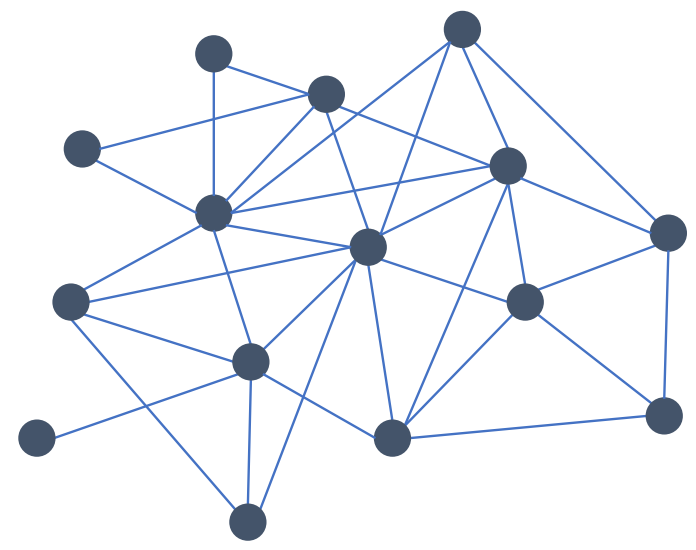
\includegraphics[width=3.8cm]{figures/Graph}
                \caption{A graph.}
            \end{figure}
        \end{column}
    \end{columns}
    
\end{frame}

\begin{frame}{Basics}
    
    \begin{block}{Definition}
        A \alert{graph} is a tuple $G = (V, E)$ where $V$ is the set of nodes and $E$ is the set of edges between these nodes. We denote an edge going from node $u \in V$ to node $v \in V$ as $(u, v) \in E$, so $E \subseteq V \times V$. The graph is \textbf{undirected} if $(u, v) \in E \Longleftrightarrow  (v, u) \in E$, otherwise it is \textbf{directed}.
    \end{block}
    
    A convenient way to represent graphs is through an \alert{adjacency matrix} $A \in \mathbb R^{|V| \times |V|}$, with $A[u, v] = 1$ if $(u, v) \in E$ and $A[u, v] = 0$ otherwise. If the graph is undirected the matrix in \emph{symmetric}. If the graph has weighted edges we have that $A[u,v] \in \mathbb R$.
    
    We also have \alert{attribute} or \alert{feature} information associated with a graph. Most often these are \emph{node-level attributes} that we represent using a real-valued matrix $\mathbf X \in \mathbb R^{d \times |V|}$, where we assume that the ordering of the nodes is consistent with the ordering in the adjacency matrix. In some cases we even associate real-valued \emph{features with entire graphs}.
    
\end{frame}

\begin{frame}{GNN real-world applications}

    GNNs are used for one of three tasks:
    \begin{itemize}[topsep=4pt,itemsep=8pt]
        \item[{$\bullet$}] {\makebox[3.3cm][l]{\alert{\emph{node classification}}:} predict the label of a given node}\\
        \quad $\longrightarrow$ \; E.g., predicting whether a user is a bot in a social network
        
        \item[{$\bullet$}] {\makebox[3.3cm][l]{\alert{\emph{edge prediction}}:}
        infer the edges between nodes in a graph}\\ 
        %predict if there exists an edge between two nodes}\\
        \quad $\longrightarrow$ \; E.g., content recommendation in online platforms, predicting drug side-effects, or inferring new facts in a relational databases
        
        \item[{$\bullet$}] {\makebox[3.3cm][l]{\alert{\emph{graph classification}}:} make independent predictions specific to each graph}\\
        \quad $\longrightarrow$ \; E.g., property prediction based on molecular graph structures
    \end{itemize}

\end{frame}

{\putbgdark
\begin{frame}[standout]
	\begin{center}
		\Large \uncover<+->{Thank you for your attention!}
		
		\Huge\uncover<+->{\Smiley}
	\end{center}
\end{frame}
}

\begin{frame}[allowframebreaks]{}

	\nocite{*}
	\printbibliography

\end{frame}

\end{document}